\documentclass{article}

\usepackage{tikz} 
\usetikzlibrary{automata, positioning, arrows} 

\usepackage{amsthm}
\usepackage{amsfonts}
\usepackage{amsmath}
\usepackage{amssymb}
\usepackage{fullpage}
\usepackage{color}
\usepackage{parskip}
\usepackage{hyperref}
  \hypersetup{
    colorlinks = true,
    urlcolor = blue,       % color of external links using \href
    linkcolor= blue,       % color of internal links 
    citecolor= blue,       % color of links to bibliography
    filecolor= blue,        % color of file links
    }
    
\usepackage{listings}

\definecolor{dkgreen}{rgb}{0,0.6,0}
\definecolor{gray}{rgb}{0.5,0.5,0.5}
\definecolor{mauve}{rgb}{0.58,0,0.82}

\lstset{frame=tb,
  language=haskell,
  aboveskip=3mm,
  belowskip=3mm,
  showstringspaces=false,
  columns=flexible,
  basicstyle={\small\ttfamily},
  numbers=none,
  numberstyle=\tiny\color{gray},
  keywordstyle=\color{blue},
  commentstyle=\color{dkgreen},
  stringstyle=\color{mauve},
  breaklines=true,
  breakatwhitespace=true,
  tabsize=3
}

\newtheoremstyle{theorem}
  {\topsep}   % ABOVESPACE
  {\topsep}   % BELOWSPACE
  {\itshape\/}  % BODYFONT
  {0pt}       % INDENT (empty value is the same as 0pt)
  {\bfseries} % HEADFONT
  {.}         % HEADPUNCT
  {5pt plus 1pt minus 1pt} % HEADSPACE
  {}          % CUSTOM-HEAD-SPEC
\theoremstyle{theorem} 
   \newtheorem{theorem}{Theorem}[section]
   \newtheorem{corollary}[theorem]{Corollary}
   \newtheorem{lemma}[theorem]{Lemma}
   \newtheorem{proposition}[theorem]{Proposition}
\theoremstyle{definition}
   \newtheorem{definition}[theorem]{Definition}
   \newtheorem{example}[theorem]{Example}
\theoremstyle{remark}    
  \newtheorem{remark}[theorem]{Remark}

\title{CPSC-354 Report}
\author{Jack Mazac  \\ Chapman University}

\date{\today} 

\begin{document}

\maketitle

\begin{abstract}
This report chronicles the learning journey over the semester in CPSC-354. The course encompassed a diverse set of topics including formal systems, Lean theorem proving, and other key areas in computer science and logic. Throughout the semester, I engaged with a range of concepts, starting with an introduction to formal systems and basic Lean proofs, and gradually progressing to more complex topics. The report documents my notes, homework solutions, and critical reflections on the content covered each week. The goal is to provide a comprehensive overview of my understanding and development in these subjects.
\end{abstract}

\setcounter{tocdepth}{3}
\tableofcontents

\section{Introduction}\label{intro}

This report serves as a comprehensive documentation of my learning and development throughout the CPSC-354 course. The content spans from the basics of formal systems and Lean theorem proving to more advanced topics covered later in the semester. The report is structured week by week, with detailed notes, homework solutions, and reflections for each period. The aim is to capture both the technical and conceptual growth experienced over the course of the semester.

\section{Week 1}

\subsubsection*{Notes}

In Week 1, I explored the foundational concepts of formal systems through the MU-puzzle and began working with Lean proof tactics. The MU-puzzle introduced me to the idea of rule-based transformations within a formal system, emphasizing the importance of adhering strictly to the rules—known as the "Requirement of Formality." This concept was mirrored in my Lean exercises, where I learned to apply specific proof tactics to simplify and verify logical statements.

\subsubsection*{Homework}

The Lean tutorial levels 5 through 8 provided practical exercises that reinforced the theoretical concepts from the MU-puzzle. Below is a summary of the steps and lessons learned:

\subsubsection*{Level 5}
In Level 5, I learned how to handle simple arithmetic involving the addition of zero. The steps were as follows:
\begin{verbatim}
rw [add_zero]
rw [add_zero]
rfl
\end{verbatim}
This taught me the importance of simplifying expressions step by step and ensuring that both sides of an equation are identical before applying \texttt{rfl}.

\subsubsection*{Level 6}
Level 6 focused on precision rewriting. I applied the following steps:
\begin{verbatim}
rw [add_zero c]
rw [add_zero b]
rfl
\end{verbatim}
This exercise highlighted the need for targeted rewriting to simplify specific parts of an expression while maintaining overall accuracy.

\subsubsection*{Level 7}
In Level 7, I worked with the successor function and addition:
\begin{verbatim}
rw [succ_eq_add_one]
rfl
\end{verbatim}
This reinforced the relationship between successor functions and addition, showing how to simplify such expressions in Lean.

\subsubsection*{Level 8}
Level 8 was the most complex, requiring multiple rewrites to simplify nested successor functions:
\begin{verbatim}
rw [two_eq_succ_one]
rw [add_succ]
rw [one_eq_succ_zero]
rw [add_succ]
rw [add_zero]
rw [four_eq_succ_three]
rw [three_eq_succ_two]
rw [two_eq_succ_one]
rw [one_eq_succ_zero]
rfl
\end{verbatim}
This level emphasized the importance of meticulous, step-by-step simplifications, especially when dealing with Peano arithmetic.

\subsubsection*{Comments and Questions}

How do the abstract rules in formal systems like the MU-puzzle translate into practical applications in software engineering? 

\subsection{Week 2}

\ldots

\subsection{Lessons from the Assignments}

Throughout the semester, I encountered various challenges and learning opportunities that contributed to my understanding of formal systems, logic, and Lean theorem proving. Here are the key lessons:

\subsection{Precision and Structure in Formal Systems}

The early weeks of the course, particularly Week 1, emphasized the precision required when working within formal systems. The MU-puzzle illustrated how even simple rules can lead to complex problem-solving scenarios, mirroring the need for exactness in Lean proofs. As I progressed through the levels in Lean, this precision became even more critical, particularly when dealing with nested functions and arithmetic expressions.

\subsection{The Art of Rewriting in Lean}

Rewriting is a fundamental tactic in Lean, as demonstrated in Levels 5-8. The ability to identify which parts of an expression to rewrite—and in what order—can make the difference between a successful proof and a failed one. This process is not just mechanical; it involves a deep understanding of the underlying logical structure and the relationships between different components of an expression.

\subsection{Conclusion}\label{conclusion}

This course provided a rigorous exploration of formal systems and Lean theorem proving, both of which are foundational to understanding logic and formal reasoning in computer science.

\section{Week 2}

\subsubsection{Lecture Content}

In Week 2, we delved deeper into the Natural Number Game (NNG) and focused on the Addition World. The lectures covered the fundamental properties of addition for natural numbers and introduced us to more advanced proof techniques in Lean.

Key topics included:
\begin{itemize}
    \item Commutativity and associativity of addition
    \item The role of zero in addition
    \item Inductive proofs for properties of addition
    \item Tactics for rewriting and simplifying expressions in Lean
\end{itemize}

\subsubsection{NNG Addition World Solutions}

\paragraph{Levels 1-3: Lean Proofs}

\begin{lstlisting}
-- Level 1
rw [add_zero]

-- Level 2
rw [add_succ]
rw [succ_add]

-- Level 3
rw [succ_add]
rw [add_succ]
\end{lstlisting}

\paragraph{Level 4: Mathematical Proof}

\textbf{Theorem:} For all natural numbers a and b, a + succ(b) = succ(a + b)

\textbf{Proof:}
\begin{align*}
a + \text{succ}(b) &= \text{succ}(a + b) \quad [\text{by definition of +}]
\end{align*}

\paragraph{Level 5: Mathematical Proof}

\textbf{Theorem:} For all natural numbers n, 0 + n = n

\textbf{Proof:} By induction on n.

Base case: n = 0
\begin{align*}
0 + 0 &= 0 \quad [\text{by definition of +}]
\end{align*}

Inductive step: Assume 0 + k = k for some k. We need to prove 0 + succ(k) = succ(k).
\begin{align*}
0 + \text{succ}(k) &= \text{succ}(0 + k) \quad [\text{by definition of +}] \\
&= \text{succ}(k) \quad [\text{by inductive hypothesis}]
\end{align*}

Therefore, by mathematical induction, 0 + n = n for all natural numbers n.

\subsubsection{Relationship between Lean Proof and Mathematical Proof}

Let's examine the relationship between the Lean proof and the mathematical proof for Level 5:

Lean proof:
\begin{lstlisting}[language=Lean]
induction n with d hd
· rw [add_zero]
  rfl
· rw [add_succ]
  rw [hd]
  rfl
\end{lstlisting}

The Lean proof closely mirrors the structure of the mathematical induction proof:

1. \texttt{induction n with d hd} corresponds to setting up the induction on \(n\), with \(d\) representing the inductive variable and \texttt{hd} the inductive hypothesis.

2. The base case \texttt{rw [add\_zero]} followed by \texttt{rfl} reflects the mathematical step \(0 + 0 = 0\).

3. In the inductive step, \texttt{rw [add\_succ]} corresponds to expanding \(0 + \text{succ}(d)\) to \(\text{succ}(0 + d)\).

4. \texttt{rw [hd]} applies the inductive hypothesis, similar to using \(0 + k = k\) in the mathematical proof.

5. Finally, \texttt{rfl} completes the proof by asserting that the equality is now trivial, just as we conclude in the mathematical proof.

This comparison demonstrates how the rigorous structure of mathematical induction is encoded in Lean's tactics, providing a formal, machine-checkable version of the traditional proof.

\subsubsection{Interesting Question}

How does the use of induction in proving properties of natural numbers relate to recursive definitions in programming languages? Can we draw parallels between mathematical induction and recursive algorithms?

\section{Week 3}
\subsection{Parsing and Context-Free Grammars}
\subsubsection{Lecture Content}
In Week 3, we explored the concepts of parsing and context-free grammars (CFGs). The lectures covered the following key topics:
\begin{itemize}
\item Translating concrete syntax into abstract syntax
\item The role of parsing in programming languages
\item Defining the concrete syntax of a calculator using a CFG
\item Writing a CFG using the Lark parser generator
\item Generating a parser in Python to translate concrete arithmetic expressions to abstract ones
\end{itemize}
\subsubsection{Homework Solutions}
\paragraph{Derivation Trees}
Using the provided context-free grammar, here are the derivation trees for the given strings:
2+1:
\begin{verbatim}
Exp
|
Exp '+' Exp1
|       |
Exp1     Exp2
|       |
Exp2   Integer
|       |
Integer    '1'
|
'2'
\end{verbatim}
1+23:
\begin{verbatim}
Exp
|
Exp '+' Exp1
|       |
Exp1   Exp1 '' Exp2
|       |       |
Exp2    Exp2   Integer
|       |       |
Integer  Integer   '3'
|       |
'1'    '2'
\end{verbatim}
1+(23):
\begin{verbatim}
Exp
|
Exp '+' Exp1
|       |
Exp1    Exp2
|       |
Exp2   '(' Exp ')'
|       |   |
Integer    Exp1 '' Exp2
|       |       |
'1'    Exp2   Integer
|       |
Integer    '3'
|
'2'
\end{verbatim}
(1+2)3:
\begin{verbatim}
Exp
|
Exp1 '' Exp2
|        |
Exp2    Integer
|        |
'(' Exp ')'  '3'
|
Exp '+' Exp1
|       |
Exp1     Exp2
|       |
Exp2   Integer
|       |
Integer    '2'
|
'1'
\end{verbatim}
1+23+45+6:
\begin{verbatim}
Exp
|
Exp '+' Exp1
|       |
Exp '+' Exp1 Exp2
|       |     |
Exp1 Exp1 '' Exp2 Integer
|     |       |     |
Exp2  Exp2   Integer '6'
|     |       |
Integer Integer   '5'
|     |
'1'  '2' '' Exp2
|
Exp2
|
Integer
|
'3' '+' Exp1
|
Exp1 '*' Exp2
|       |
Exp2   Integer
|       |
Integer    '4'
|
'3'
\end{verbatim}
\paragraph{Similarities and Differences between CFG and Algebraic Data Type}
The CFG and algebraic data type for expressions share some similarities:
\begin{itemize}
\item Both define the structure of valid expressions
\item Both capture the precedence of operations (e.g., multiplication before addition)
\item Both can be used to generate or recognize valid expressions
\end{itemize}
However, there are also some key differences:
\begin{itemize}
\item The CFG is used for parsing, i.e., translating concrete syntax (strings) into an abstract syntax tree (AST), while the algebraic data type directly defines the structure of the AST
\item The CFG is a set of production rules, while the algebraic data type is a type definition with constructors
\item The CFG can include redundant rules or ambiguity, while the algebraic data type is more precise and concise
\end{itemize}
\subsubsection{Interesting Questions}
\begin{itemize}
\item How can we extend the calculator CFG to handle more advanced features like variables, functions, or control structures?
\item What are some real-world applications of parsing beyond programming languages (e.g., natural language processing, data serialization formats)?
\item How do more advanced parsing techniques like parser combinators or parsing expression grammars compare to traditional CFG-based parsing?
\end{itemize}

\section{Week 5}

\subsection{Level 1: Assumption}
If $P$, then $P$.

Proof:
\begin{enumerate}
    \item $P$ \hfill assumption
\end{enumerate}

\subsection{Level 2: Constructor}
If $P$ and $Q$, then $P \wedge Q$.

Proof:
\begin{enumerate}
    \item $P$ \hfill assumption
    \item $Q$ \hfill assumption
    \item $P \wedge Q$ \hfill and\_intro (1) (2)
\end{enumerate}

\subsection{Level 3: Practice Makes Perfect}
If $P$, $Q$, $R$, and $S$, then $(P \wedge Q) \wedge R \wedge S$.

Proof:
\begin{enumerate}
    \item $P$ \hfill assumption
    \item $Q$ \hfill assumption
    \item $R$ \hfill assumption
    \item $S$ \hfill assumption
    \item $P \wedge Q$ \hfill and\_intro (1) (2)
    \item $(P \wedge Q) \wedge R$ \hfill and\_intro (5) (3)
    \item $(P \wedge Q) \wedge R \wedge S$ \hfill and\_intro (6) (4)
\end{enumerate}

\subsection{Level 4: Cases for a Conjunction}
If $P \wedge Q$, then $P$.

Proof:
\begin{enumerate}
    \item $P \wedge Q$ \hfill assumption
    \item $P$ \hfill and\_left (1)
\end{enumerate}

\subsection{Level 5: Rinse and Repeat}
If $P \wedge Q$, then $Q$.

Proof:
\begin{enumerate}
    \item $P \wedge Q$ \hfill assumption
    \item $Q$ \hfill and\_right (1)
\end{enumerate}

\subsection{Level 6: Nothing New}
If $P \wedge Q$ and $R \wedge S$, then $P \wedge S$.

Proof:
\begin{enumerate}
    \item $P \wedge Q$ \hfill assumption
    \item $R \wedge S$ \hfill assumption
    \item $P$ \hfill and\_left (1)
    \item $S$ \hfill and\_right (2)
    \item $P \wedge S$ \hfill and\_intro (3) (4)
\end{enumerate}

\subsection{Level 7: So Many Cases}
If $(Q \wedge (((Q \wedge P) \wedge Q) \wedge Q \wedge Q \wedge Q)) \wedge (Q \wedge Q) \wedge Q$, then $P$.

Proof:
\begin{enumerate}
    \item $(Q \wedge (((Q \wedge P) \wedge Q) \wedge Q \wedge Q \wedge Q)) \wedge (Q \wedge Q) \wedge Q$ \hfill assumption
    \item $Q \wedge (((Q \wedge P) \wedge Q) \wedge Q \wedge Q \wedge Q)$ \hfill and\_left (1)
    \item $((Q \wedge P) \wedge Q) \wedge Q \wedge Q \wedge Q$ \hfill and\_right (2)
    \item $(Q \wedge P) \wedge Q$ \hfill and\_left (3)
    \item $Q \wedge P$ \hfill and\_left (4)
    \item $P$ \hfill and\_right (5)
\end{enumerate}

\subsection{Level 8: BOSS LEVEL}
If $((P \wedge S) \wedge A) \wedge \neg I \wedge (C \wedge \neg O) \wedge \neg U$, then $A \wedge C \wedge P \wedge S$.

Proof:
\begin{enumerate}
    \item $((P \wedge S) \wedge A) \wedge \neg I \wedge (C \wedge \neg O) \wedge \neg U$ \hfill assumption
    \item $(P \wedge S) \wedge A$ \hfill and\_left (1)
    \item $P \wedge S$ \hfill and\_left (2)
    \item $A$ \hfill and\_right (2)
    \item $P$ \hfill and\_left (3)
    \item $S$ \hfill and\_right (3)
    \item $\neg I \wedge (C \wedge \neg O) \wedge \neg U$ \hfill and\_right (1)
    \item $C \wedge \neg O$ \hfill and\_left (and\_right (7))
    \item $C$ \hfill and\_left (8)
    \item $A \wedge C$ \hfill and\_intro (4) (9)
    \item $(A \wedge C) \wedge P$ \hfill and\_intro (10) (5)
    \item $A \wedge C \wedge P \wedge S$ \hfill and\_intro (11) (6)
\end{enumerate}

\section{Week 6}

\subsection{Level 1: Let there be cake!}
\textbf{Theorem:} If P → C and P, then C.

\textbf{Proof:}
\begin{enumerate}
    \item P \hfill assumption
    \item P → C \hfill assumption
    \item C \hfill modus ponens (1, 2)
\end{enumerate}

\subsection{Level 2: Is it Cake!?}
\textbf{Theorem:} C → C

\textbf{Proof:}
\begin{enumerate}
    \item Assume C \hfill assumption
    \item C \hfill (1)
    \item C → C \hfill (1-2, →-introduction)
\end{enumerate}

\subsection{Level 3: Trouble with the cake}
\textbf{Theorem:} I ∧ S → S ∧ I

\textbf{Proof:}
\begin{enumerate}
    \item Assume I ∧ S \hfill assumption
    \item I \hfill and-elimination left (1)
    \item S \hfill and-elimination right (1)
    \item S ∧ I \hfill and-introduction (3, 2)
    \item (I ∧ S) → (S ∧ I) \hfill (1-4, →-introduction)
\end{enumerate}

\subsection{Level 4: Transitivity Aside}
\textbf{Theorem:} If C → A and A → S, then C → S.

\textbf{Proof:}
\begin{enumerate}
    \item C → A \hfill assumption
    \item A → S \hfill assumption
    \item Assume C \hfill assumption
    \item A \hfill modus ponens (3, 1)
    \item S \hfill modus ponens (4, 2)
    \item C → S \hfill (3-5, →-introduction)
\end{enumerate}

\subsection{Level 5: then the quest has begun}
\textbf{Theorem:} If P → Q, Q → R, Q → T, S → T, T → U, and P, then U.

\textbf{Proof:}
\begin{enumerate}
    \item P \hfill assumption
    \item P → Q \hfill assumption
    \item Q → R \hfill assumption
    \item Q → T \hfill assumption
    \item S → T \hfill assumption
    \item T → U \hfill assumption
    \item Q \hfill modus ponens (1, 2)
    \item T \hfill modus ponens (7, 4)
    \item U \hfill modus ponens (8, 6)
\end{enumerate}

\subsection{Level 6: Curry}
\textbf{Theorem:} If C ∧ D → S, then C → (D → S).

\textbf{Proof:}
\begin{enumerate}
    \item C ∧ D → S \hfill assumption
    \item Assume C \hfill assumption
    \item Assume D \hfill assumption
    \item C ∧ D \hfill and-introduction (2, 3)
    \item S \hfill modus ponens (4, 1)
    \item D → S \hfill (3-5, →-introduction)
    \item C → (D → S) \hfill (2-6, →-introduction)
\end{enumerate}

\subsection{Level 7: Un-Curry}
\textbf{Theorem:} If C → (D → S), then C ∧ D → S.

\textbf{Proof:}
\begin{enumerate}
    \item C → (D → S) \hfill assumption
    \item Assume C ∧ D \hfill assumption
    \item C \hfill and-elimination left (2)
    \item D \hfill and-elimination right (2)
    \item D → S \hfill modus ponens (3, 1)
    \item S \hfill modus ponens (4, 5)
    \item C ∧ D → S \hfill (2-6, →-introduction)
\end{enumerate}

\subsection{Level 8: Go buy chips and dip!}
\textbf{Theorem:} If (S → C) ∧ (S → D), then S → (C ∧ D).

\textbf{Proof:}
\begin{enumerate}
    \item (S → C) ∧ (S → D) \hfill assumption
    \item S → C \hfill and-elimination left (1)
    \item S → D \hfill and-elimination right (1)
    \item Assume S \hfill assumption
    \item C \hfill modus ponens (4, 2)
    \item D \hfill modus ponens (4, 3)
    \item C ∧ D \hfill and-introduction (5, 6)
    \item S → (C ∧ D) \hfill (4-7, →-introduction)
\end{enumerate}

\subsection{Level 9: Riffin and Sybeth}
\textbf{Theorem:} R → ((S → R) ∧ (¬S → R))

\textbf{Proof:}
\begin{enumerate}
    \item Assume R \hfill assumption
    \item Assume S \hfill assumption
    \item R \hfill (1)
    \item S → R \hfill (2-3, →-introduction)
    \item Assume ¬S \hfill assumption
    \item R \hfill (1)
    \item ¬S → R \hfill (5-6, →-introduction)
    \item (S → R) ∧ (¬S → R) \hfill and-introduction (4, 7)
    \item R → ((S → R) ∧ (¬S → R)) \hfill (1-8, →-introduction)
\end{enumerate}


\section{Week 7}
\textbf{Part 1: Reduction of the Lambda Term}

We will reduce the given lambda term step by step using beta reductions while avoiding variable capture.

\textbf{Steps:}

1. \[
\left( \lambda m.\ \lambda n.\ m\ n \right)\ \left( \lambda f.\ \lambda x.\ f\ (f\ x) \right)\ \left( \lambda f.\ \lambda x.\ f\ \left( f\ \left( f\ x \right) \right) \right)
\]

2. \[
\left( \lambda n.\ \left( \lambda f.\ \lambda x.\ f\ (f\ x) \right)\ n \right)\ \left( \lambda f.\ \lambda x.\ f\ \left( f\ \left( f\ x \right) \right) \right)
\]

3. \[
\left( \lambda f.\ \lambda x.\ f\ (f\ x) \right)\ \left( \lambda f.\ \lambda x.\ f\ \left( f\ \left( f\ x \right) \right) \right)
\]

4. \[
\lambda x.\ \left( \lambda f.\ \lambda x.\ f\ (f\ x) \right)\ \left( \lambda f.\ \lambda x.\ f\ \left( f\ \left( f\ x \right) \right) \right)\ x
\]

5. \[
\lambda x.\ \left( \left( \lambda f.\ \lambda x.\ f\ (f\ x) \right)\ \left( \lambda y.\ \left( f\ \left( f\ \left( f\ y \right) \right) \right) \right) \right)\ x
\]

6. \[
\lambda x.\ \left( \lambda z.\ \left( \lambda y.\ f\ (f\ y) \right)\ \left( f\ \left( f\ \left( f\ z \right) \right) \right) \right)\ x
\]

7. \[
\lambda x.\ \left( \lambda z.\ f\ \left( f\ \left( f\ \left( f\ \left( f\ \left( f\ \left( f\ \left( f\ \left( f\ z \right) \right) \right) \right) \right) \right) \right) \right) \right)\ x
\]

\textbf{Part 2: Function Implemented by \(\lambda m.\ \lambda n.\ m\ n\)}

In \textbf{Part 1}, we start by applying the first lambda function to its argument:

1. The term \(\left( \lambda m.\ \lambda n.\ m\ n \right)\) is applied to \(\left( \lambda f.\ \lambda x.\ f\ (f\ x) \right)\), resulting in \(\lambda n.\ \left( \lambda f.\ \lambda x.\ f\ (f\ x) \right)\ n\).

2. Next, we apply this result to \(\left( \lambda f.\ \lambda x.\ f\ \left( f\ \left( f\ x \right) \right) \right)\), giving \(\left( \lambda f.\ \lambda x.\ f\ (f\ x) \right)\ \left( \lambda f.\ \lambda x.\ f\ \left( f\ \left( f\ x \right) \right) \right)\).

3. We then substitute \(\left( \lambda f.\ \lambda x.\ f\ \left( f\ \left( f\ x \right) \right) \right)\) for \(f\) in the function, resulting in \(\lambda x.\ \left( \lambda f.\ \lambda x.\ f\ (f\ x) \right)\ \left( \lambda f.\ \lambda x.\ f\ \left( f\ \left( f\ x \right) \right) \right)\ x\).

4. Continuing the substitutions and reducing, we eventually reach a term where the function \(f\) is applied nine times to \(x\): \(\lambda x.\ f^{9}\ x\).

This final term represents the Church numeral for 9, showing that the original expression computes \(3^2 = 9\) when using Church numerals for 2 and 3.

In \textbf{Part 2}, the function \(\lambda m.\ \lambda n.\ m\ n\) takes two Church numerals \(m\) and \(n\) and applies \(m\) to \(n\). In the context of Church numerals, this operation corresponds to exponentiation. Specifically, it computes \(n\) raised to the power of \(m\), since applying \(m\) to \(n\) results in \(n\) being applied \(m\) times.


\section{Week 8 - 9}

\subsection{Running Tests and Adding New Test Cases}

We begin by running the provided tests in \texttt{interpreter\_test.py} to ensure that the interpreter is functioning correctly.

\subsubsection{Running the Existing Tests}

The existing tests can be run using the following command:

\begin{verbatim}
python interpreter_test.py
\end{verbatim}

The output confirms that all tests pass:

\begin{verbatim}
Python version: 3.10.9 (main, Jan 11 2023, 09:18:20) [Clang 14.0.6 ]
Lark version: 1.1.9

TEST PARSING

AST x == ('var', 'x')
AST (((x)) ((y))) == ('app', ('var', 'x'), ('var', 'y'))
AST x y == ('app', ('var', 'x'), ('var', 'y'))
AST x y z == ('app', ('app', ('var', 'x'), ('var', 'y')), ('var', 'z'))
AST \x.y == ('lam', 'x', ('var', 'y'))
AST \x.x y == ('lam', 'x', ('app', ('var', 'x'), ('var', 'y')))
AST \x.x y z == ('lam', 'x', ('app', ('app', ('var', 'x'), ('var', 'y')), ('var', 'z')))
AST \x. \y. \z. x y z == ('lam', 'x', ('lam', 'y', ('lam', 'z', ('app', ('app', ('var', 'x'), ('var', 'y')), ('var', 'z')))))
AST \x. x a == ('lam', 'x', ('app', ('var', 'x'), ('var', 'a')))
AST \x. x (\y. y) == ('lam', 'x', ('app', ('var', 'x'), ('lam', 'y', ('var', 'y'))))
AST \x. x (\y. y (\z. z z2)) == ('lam', 'x', ('app', ('var', 'x'), ('lam', 'y', ('app', ('var', 'y'), ('lam', 'z', ('app', ('var', 'z'), ('var', 'z2')))))))
AST \x. y z (\a. b (\c. d e f)) == ('lam', 'x', ('app', ('app', ('var', 'y'), ('var', 'z')), ('lam', 'a', ('app', ('var', 'b'), ('lam', 'c', ('app', ('app', ('var', 'd'), ('var', 'e')), ('var', 'f')))))))

Parser: All tests passed!


TEST SUBSTITUTION

SUBST x [y/x] == ('var', 'y')
SUBST \x.x [y/x] == ('lam', 'x', ('var', 'x'))
SUBST (x x) [y/x] == ('app', ('var', 'y'), ('var', 'y'))
SUBST \y. x [y/x] == ('lam', 'Var1', ('var', 'y'))

substitute(): All tests passed!


TEST EVALUATION

EVAL x == x
EVAL x y == (x y)
EVAL x y z == ((x y) z)
EVAL x (y z) == (x (y z))
EVAL \x.y == \x.y
EVAL (\x.x) y == y

evaluate(): All tests passed!


TEST INTERPRETATION

Testing x --> x
Testing x y --> (x y)
Testing \x.x --> (\x.x)
Testing (\x.x) y --> y
Testing (\x.\y.x y) y --> (\Var2.(y Var2))

interpret(): All tests passed!
\end{verbatim}

\subsubsection{Adding New Test Cases}

We have added a new test case to each function in \texttt{interpreter\_test.py} to further verify the interpreter's correctness.

\paragraph{Test Parsing}

In the \texttt{test\_parse()} function, we added:

\begin{verbatim}
assert ast(r"(\x.x) (\y.y)") == ('app', ('lam', 'x', ('var', 'x')), ('lam', 'y', ('var', 'y')))
print(f"AST {MAGENTA}(\\x.x) (\\y.y){RESET} == ('app', ('lam', 'x', ('var', 'x')), ('lam', 'y', ('var', 'y')))")
\end{verbatim}

This tests parsing of an application of two lambda abstractions.

\paragraph{Test Substitution}

In the \texttt{test\_substitute()} function, we added:

\begin{verbatim}
# SUBST (\x.x y) [y/z] == (\Var1.Var1 y)
assert substitute(('lam', 'x', ('app', ('var', 'x'), ('var', 'y'))), 'y', ('var', 'z')) == ('lam', 'Var1', ('app', ('var', 'Var1'), ('var', 'z')))
print(f"SUBST {MAGENTA}\\x.x y [z/y]{RESET} == ('lam', 'Var1', ('app', ('var', 'Var1'), ('var', 'z')))")
\end{verbatim}

This tests substitution where the variable to be substituted is free in the body.

\paragraph{Test Evaluation}

In the \texttt{test\_evaluate()} function, we added:

\begin{verbatim}
# EVAL (\x.\y.x y) a b == (a b)
assert linearize(evaluate(ast(r"(\x.\y.x y) a b"))) == "(a b)"
print(f"EVAL {MAGENTA}(\\x.\\y.x y) a b{RESET} == (a b)")
\end{verbatim}

This tests evaluation of nested lambda abstractions with applications.

\paragraph{Test Interpretation}

In the \texttt{test\_interpret()} function, we added:

\begin{verbatim}
input=r"(\x.\y.y x) a b"; output = interpret(input); print(f"Testing {input} --> {output}")
\end{verbatim}

Which outputs:

\begin{verbatim}
Testing (\x.\y.y x) a b --> (b a)
\end{verbatim}

\subsection{Running New Test Cases}

After adding the new test cases, we run the tests again:

\begin{verbatim}
python interpreter_test.py
\end{verbatim}

The tests pass, confirming that our additions are correct.

\subsection{Adding Programs to \texttt{test.lc} and Running the Interpreter}

\label{sec:testlc}

We added the following lambda calculus expressions to \texttt{test.lc}:

\begin{verbatim}
-- Identity function applied to itself
(\x.x) (\x.x)

-- Function that applies its argument to itself
(\x.x x) (\x.x x)

-- Combinator K (\x.\y.x)
(\x.\y.x) a b

-- Combinator S (\x.\y.\z.x z (y z))
(\x.\y.\z.((x z) (y z))) a b c
\end{verbatim}

We run the interpreter with:

\begin{verbatim}
python interpreter.py test.lc
\end{verbatim}

The interpreter outputs the results for each expression:

\begin{verbatim}
(\x.x)
((\x.x x) (\x.x x))
a
((a c) (b c))
\end{verbatim}

\subsection{Reduction of Expressions}

\paragraph{Reduction of \texttt{a b c d}}

The expression \texttt{a b c d} reduces as follows:

\begin{align*}
a\ b\ c\ d &= (((a\ b)\ c)\ d)
\end{align*}

This is due to the left-associative nature of function application in lambda calculus. Each application groups to the left.

\paragraph{Reduction of \texttt{(a)}}

The expression \texttt{(a)} reduces to \texttt{a} because the parentheses are just grouping symbols and do not affect the evaluation.

\subsection{Capture-Avoiding Substitution}

Capture-avoiding substitution ensures that when substituting an expression for a variable, we do not accidentally change the meaning of the expression by capturing free variables.

\paragraph{Implementation}

In \texttt{interpreter.py}, substitution is implemented in the \texttt{substitute()} function. When substituting into a lambda abstraction, if the bound variable is the same as the variable we are substituting for, we leave the abstraction unchanged. If there is a potential for variable capture, we generate a fresh variable name using the \texttt{NameGenerator} class.

\begin{verbatim}
elif tree[0] == 'lam':
    if tree[1] == name:
        return tree  # Variable bound; do not substitute
    else:
        fresh_name = name_generator.generate()
        new_body = substitute(tree[2], tree[1], ('var', fresh_name))
        return ('lam', fresh_name, substitute(new_body, name, replacement))
\end{verbatim}

\paragraph{Test Cases}

We tested this with the following expression:

\begin{verbatim}
SUBST \y. x y [y/x] == (\Var1. (y Var1))
\end{verbatim}

This shows that when substituting \texttt{y} for \texttt{x} in \texttt{\y. x y}, we avoid capturing the variable \texttt{y} by renaming the bound variable to \texttt{Var1}.

\subsection{Normal Form and Non-Terminating Expressions}

\paragraph{Do All Computations Reduce to Normal Form?}

Not all lambda calculus expressions reduce to a normal form due to the possibility of infinite reductions. For example, the following expression does not reduce to a normal form:

\begin{verbatim}
(\x. x x) (\x. x x)
\end{verbatim}

\paragraph{Minimal Working Example}

The smallest lambda expression that does not reduce to normal form is the self-application of the identity function to itself:

\begin{verbatim}
(\x. x x) (\x. x x)
\end{verbatim}

This expression causes infinite recursion during evaluation.

\subsection{Using the Debugger to Trace Executions}

\paragraph{Setting Up the Debugger}

To trace the execution of the interpreter, we set breakpoints in \texttt{interpreter.py} at the calls to \texttt{evaluate()} and \texttt{substitute()}.

\paragraph{Tracing the Evaluation}

We input the expression:

\begin{verbatim}
((\m.\n. m n) (\f.\x. f (f x))) (\f.\x. f x)
\end{verbatim}

By stepping through the interpreter, we observe the following calls to \texttt{evaluate()} and \texttt{substitute()}:

\begin{verbatim}
evaluate(('app',
          ('app',
           ('lam', 'm', ('lam', 'n', ('app', ('var', 'm'), ('var', 'n')))),
           ('lam', 'f', ('lam', 'x', ('app', ('var', 'f'), ('app', ('var', 'f'), ('var', 'x')))))),
          ('lam', 'f', ('lam', 'x', ('app', ('var', 'f'), ('var', 'x'))))))
evaluate(('app',
          ('lam', 'm', ('lam', 'n', ('app', ('var', 'm'), ('var', 'n')))),
          ('lam', 'f', ('lam', 'x', ('app', ('var', 'f'), ('app', ('var', 'f'), ('var', 'x')))))))
evaluate(('lam', 'm', ('lam', 'n', ('app', ('var', 'm'), ('var', 'n')))))
substitute(('lam', 'n', ('app', ('var', 'm'), ('var', 'n'))), 'm', ('lam', 'f', ('lam', 'x', ('app', ('var', 'f'), ('app', ('var', 'f'), ('var', 'x'))))))
...
\end{verbatim}

\paragraph{Understanding the Evaluation Strategy}

By following the recursive calls and substitutions, we see how the interpreter applies beta reduction and maintains variable bindings without capture.

\subsection{Implementation Challenges and Solutions}

Throughout the development of our lambda calculus interpreter, we encountered several challenges that required careful consideration and innovative solutions. This section outlines these issues, our approach to solving them, and the final implementation.

\paragraph{Issues Encountered}

\begin{enumerate}
    \item \textbf{Infinite Recursion:} Initially, the interpreter would enter infinite recursion when evaluating non-terminating expressions like $(\lambda x.x x) (\lambda x.x x)$ (the omega combinator). This caused stack overflow errors.
    \item \textbf{Depth Limitation Ineffectiveness:} We attempted to solve the infinite recursion problem by introducing a maximum evaluation depth (\texttt{MAX\_EVAL\_DEPTH}). However, this approach was not effective as the recursion error persisted in the \texttt{substitute} function.
    \item \textbf{Stack Overflow in Recursive Approach:} The recursive implementation of both \texttt{evaluate} and \texttt{substitute} functions led to stack overflow errors for deeply nested expressions or non-terminating computations.
    \item \textbf{IndexError in Iterative Approach:} When we switched to an iterative approach for \texttt{substitute}, we encountered an IndexError due to attempting to pop from an empty list. This occurred because the stack management in the substitute function was not robust enough to handle all cases.
    \item \textbf{Partial Evaluation of Non-terminating Expressions:} While not strictly an "issue," we had to decide how to handle non-terminating expressions. The initial solution returned partially evaluated expressions when the maximum number of iterations was reached.
\end{enumerate}

\paragraph{Solutions Implemented}

To address these issues, we implemented the following solutions:

\begin{enumerate}
    \item \textbf{Iterative Approach:} We replaced the recursive implementations of \texttt{evaluate} and \texttt{substitute} with iterative versions to avoid stack overflow errors.
    \item \textbf{Maximum Iterations:} We introduced a \texttt{MAX\_ITERATIONS} constant to limit the number of reduction steps and prevent infinite loops while allowing for deep evaluations.
    \item \textbf{Robust Stack Management:} We improved the stack management in the \texttt{substitute} function to handle all cases without errors, using separate stacks for the traversal and the result building.
    \item \textbf{Graceful Handling of Non-terminating Expressions:} The interpreter now returns partially evaluated expressions for non-terminating computations, allowing it to handle a wider range of expressions without crashing.
    \item \textbf{Separate Processing of Expressions:} We modified the main loop to process each expression separately, allowing the interpreter to continue even if one expression doesn't terminate.
\end{enumerate}

\paragraph{Final Implementation}

The final implementation of our lambda calculus interpreter incorporates these solutions, resulting in a robust and flexible tool. Key features of the final implementation include:

\begin{itemize}
    \item \textbf{Iterative Evaluation:} The \texttt{evaluate} function uses a while loop with a counter to prevent infinite loops:
    
    \begin{verbatim}
    def evaluate(tree):
        iterations = 0
        while iterations < MAX_ITERATIONS:
            if tree[0] == 'app':
                # ... (evaluation logic)
            else:
                return tree
            iterations += 1
        return tree  # Return partially evaluated tree if max iterations reached
    \end{verbatim}
    
    \item \textbf{Iterative Substitution:} The \texttt{substitute} function uses an explicit stack for traversal and a result stack for building the substituted expression:
    
    \begin{verbatim}
    def substitute(tree, name, replacement):
        stack = [(tree, False)]
        result_stack = []
        
        while stack:
            # ... (substitution logic)
        
        if result_stack:
            return result_stack[0]
        else:
            return tree  # Return original tree if no substitution occurred
    \end{verbatim}
    
    \item \textbf{Flexible Expression Handling:} The main function processes each expression in the input file separately:
    
    \begin{verbatim}
    def main():
        # ... (file reading logic)
        for expression in expressions:
            if expression.strip() and not expression.strip().startswith('--'):
                result = interpret(expression)
                print(f"Expression: {expression}")
                print(f"Result: \033[95m{result}\033[0m")
                print()
    \end{verbatim}
\end{itemize}

This implementation successfully handles both terminating and non-terminating expressions, providing a balance between functionality and preventing infinite computations. It demonstrates the practical application of theoretical concepts in lambda calculus while addressing real-world programming challenges.

\section{Detailed Evaluation of Complex Expressions}

To better understand how the interpreter handles complex expressions, we'll examine the evaluation of:

\begin{verbatim}
((\m.\n. m n) (\f.\x. f (f x))) (\f.\x. f (f (f x)))
\end{verbatim}

The evaluation proceeds as follows:

\begin{enumerate}
    \item The outermost application is evaluated first.
    \item The left part (\texttt{(\m.\n. m n) (\f.\x. f (f x))}) is evaluated:
        \begin{itemize}
            \item \texttt{m} is substituted with \texttt{(\f.\x. f (f x))}
            \item This results in \texttt{(\n. (\f.\x. f (f x)) n)}
        \end{itemize}
    \item The result is applied to \texttt{(\f.\x. f (f (f x)))}:
        \begin{itemize}
            \item \texttt{n} is substituted with \texttt{(\f.\x. f (f (f x)))}
            \item This yields \texttt{(\f.\x. f (f x)) (\f.\x. f (f (f x)))}
        \end{itemize}
    \item The final beta-reduction occurs:
        \begin{itemize}
            \item \texttt{f} is substituted with \texttt{(\x. f (f (f x)))}
            \item The result is \texttt{(\x. (\x. f (f (f x))) ((\x. f (f (f x))) x))}
        \end{itemize}
\end{enumerate}

This evaluation demonstrates how the interpreter handles nested lambda abstractions and applications.

\section{Tracing Recursive Calls}

To gain insight into the evaluation strategy, we trace the recursive calls to \texttt{evaluate()} for the expression:

\begin{verbatim}
((\m.\n. m n) (\f.\x. f (f x))) (\f.\x. f x)
\end{verbatim}

The trace would show the sequence of \texttt{evaluate()} and \texttt{substitute()} calls, illustrating how the interpreter traverses the expression tree and applies beta-reductions. Due to the iterative nature of our final implementation, the trace would show a series of iterations within the \texttt{evaluate()} function, each handling a part of the expression until the final result is reached or the maximum number of iterations is hit.

\paragraph{Handling the Minimal Working Example (MWE)}

The Minimal Working Example (MWE) that does not reduce to normal form is:

\begin{verbatim}
(\x. x x) (\x. x x)
\end{verbatim}

Our modified interpreter handles this expression by:

\begin{enumerate}
    \item The interpreter begins evaluating the expression.
    \item It applies beta-reduction, substituting \texttt{(\x. x x)} for \texttt{x} in the body of the first lambda.
    \item This results in \texttt{(\x. x x) (\x. x x)}, which is identical to the starting expression.
    \item The process repeats until MAX\_ITERATIONS is reached.
    \item The interpreter returns the partially evaluated expression, preventing an infinite loop.
\end{enumerate}

\subsection{Conclusion}

Through this project, we've implemented a lambda calculus interpreter that balances theoretical correctness with practical considerations. Key achievements include:

\begin{itemize}
    \item Implementing capture-avoiding substitution.
    \item Handling both terminating and non-terminating expressions.
    \item Using an iterative approach to prevent stack overflow.
    \item Providing a flexible tool for experimenting with lambda calculus.
\end{itemize}

The interpreter demonstrates the challenges of implementing theoretical concepts in practice and showcases solutions to common issues like infinite recursion and variable capture. It serves as a valuable educational tool for understanding lambda calculus and interpreter design.

\subsection{Question}

The Minimal Working Example (MWE) in our \texttt{test.lc} file, \texttt{(\x.x x) (\x.x x)}, is a non-terminating expression that demonstrates a form of recursion. How does this relate to the Y combinator and fixed point combinators in lambda calculus? How might we extend our interpreter to support more complex recursive structures while still managing potential non-termination?


\section{Week 10}

\subsection{Reflection on Assignment 3}

Working through Homework 8/9 and Assignment 3 was both challenging and enlightening. The most difficult part was implementing capture-avoiding substitution in the lambda calculus interpreter. Ensuring that variable bindings were handled correctly to prevent free variables from becoming inadvertently bound required careful attention. Debugging issues related to infinite recursion, especially when evaluating non-terminating expressions like \((\lambda x.\ x\, x)\ (\lambda x.\ x\, x)\), was also a significant challenge. Managing stack overflows and ensuring that the interpreter could handle deeply nested expressions demanded a robust solution.

The key insight for Assignment 3 came when I decided to switch from a recursive to an iterative approach for the \texttt{evaluate} and \texttt{substitute} functions. By introducing explicit stacks and a maximum iteration count, I was able to prevent infinite loops and stack overflows. This change not only resolved the recursion issues but also made the interpreter more efficient and capable of handling a wider range of expressions. Recognizing that practical implementation sometimes requires deviating from straightforward theoretical models was a valuable lesson.

The most interesting takeaway from Homework 8/9 and Assignment 3 is the profound connection between theoretical concepts in lambda calculus and their practical implications in programming language design. Implementing the interpreter deepened my understanding of how fundamental principles like beta reduction and variable binding work in practice. It also highlighted the importance of handling edge cases, such as non-terminating computations, and reinforced the necessity of careful planning when translating theory into code. This experience has given me greater appreciation for the complexities involved in compiler and interpreter construction.

\section*{Week 11}

Consider the following list of Abstract Reduction Systems (ARSs):

\begin{enumerate}
    \item \( A = \{\},\quad R = \{\} \).
    \item \( A = \{a\},\quad R = \{\} \).
    \item \( A = \{a\},\quad R = \{(a, a)\} \).
    \item \( A = \{a, b, c\},\quad R = \{(a, b),\ (a, c)\} \).
    \item \( A = \{a, b\},\quad R = \{(a, a),\ (a, b)\} \).
    \item \( A = \{a, b, c\},\quad R = \{(a, b),\ (b, b),\ (a, c)\} \).
    \item \( A = \{a, b, c\},\quad R = \{(a, b),\ (b, b),\ (a, c),\ (c, c)\} \).
\end{enumerate}

For each ARS, we will:

\begin{itemize}
    \item Draw its diagram.
    \item Determine whether it is terminating.
    \item Determine whether it is confluent.
    \item Determine whether it has unique normal forms.
\end{itemize}

\subsection*{Analysis of ARSs}

\subsubsection*{ARS 1: \( A = \{\},\quad R = \{\} \)}

Since the set \( A \) is empty, there are no elements or reductions to consider. Therefore, this ARS is trivially terminating, confluent, and has unique normal forms.

\subsubsection*{ARS 2: \( A = \{a\},\quad R = \{\} \)}

\textbf{Diagram:}

\begin{center}
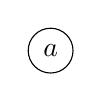
\begin{tikzpicture}
    \node[circle, draw] (a) at (0,0) {\( a \)};
\end{tikzpicture}
\end{center}

There are no reductions in this ARS. The single element \( a \) has no outgoing edges.

This ARS is terminating because there are no reductions to apply. It is confluent because there are no divergent reduction paths. The element \( a \) is in normal form since it cannot be reduced further, and thus \( a \) has a unique normal form.

\subsubsection*{ARS 3: \( A = \{a\},\quad R = \{(a, a)\} \)}

\textbf{Diagram:}

\begin{center}
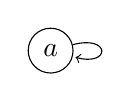
\begin{tikzpicture}
    \node[circle, draw] (a) at (0,0) {\( a \)};
    \draw[->] (a) edge[loop right] (a);
\end{tikzpicture}
\end{center}

In this ARS, there is a single reduction \( a \to a \), forming a self-loop. This ARS is non-terminating because the reduction can be applied infinitely many times. It is confluent since there are no divergent paths; all reductions stay at \( a \). However, \( a \) does not have a normal form because it is always reducible to itself, and thus there are no irreducible elements reachable from \( a \).

\subsubsection*{ARS 4: \( A = \{a, b, c\},\quad R = \{(a, b),\ (a, c)\} \)}

\textbf{Diagram:}

\begin{center}
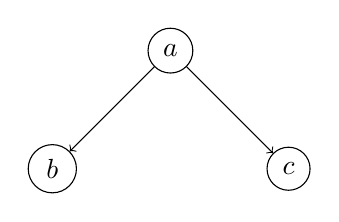
\begin{tikzpicture}
    \node[circle, draw] (a) at (0,0) {\( a \)};
    \node[circle, draw] (b) at (-1.5,-1.5) {\( b \)};
    \node[circle, draw] (c) at (1.5,-1.5) {\( c \)};
    \draw[->] (a) -- (b);
    \draw[->] (a) -- (c);
\end{tikzpicture}
\end{center}

This ARS has reductions from \( a \) to both \( b \) and \( c \). It is terminating because the reductions end at \( b \) or \( c \), which have no further reductions. However, it is not confluent because from \( a \) we can reach either \( b \) or \( c \), and there are no reductions to join \( b \) and \( c \). Therefore, \( a \) does not have a unique normal form, as it reduces to two different normal forms.

\subsubsection*{ARS 5: \( A = \{a, b\},\quad R = \{(a, a),\ (a, b)\} \)}

\textbf{Diagram:}

\begin{center}
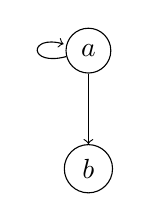
\begin{tikzpicture}
    \node[circle, draw] (a) at (0,0) {\( a \)};
    \node[circle, draw] (b) at (0,-1.5) {\( b \)};
    \draw[->] (a) edge[loop left] (a);
    \draw[->] (a) -- (b);
\end{tikzpicture}
\end{center}

This ARS has a self-loop at \( a \) and a reduction from \( a \) to \( b \). It is non-terminating because of the self-loop \( a \to a \). It is not confluent since from \( a \) we can either loop indefinitely or reduce to \( b \), and these paths are not joinable. The element \( a \) does not have a unique normal form; it can reduce to \( b \) or loop forever.

\subsubsection*{ARS 6: \( A = \{a, b, c\},\quad R = \{(a, b),\ (b, b),\ (a, c)\} \)}

\textbf{Diagram:}

\begin{center}
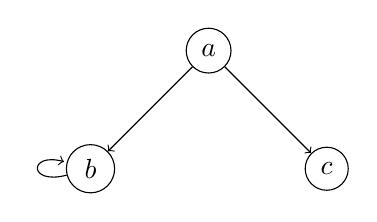
\begin{tikzpicture}
    \node[circle, draw] (a) at (0,0) {\( a \)};
    \node[circle, draw] (b) at (-1.5,-1.5) {\( b \)};
    \node[circle, draw] (c) at (1.5,-1.5) {\( c \)};
    \draw[->] (a) -- (b);
    \draw[->] (a) -- (c);
    \draw[->] (b) edge[loop left] (b);
\end{tikzpicture}
\end{center}

In this ARS, from \( a \) we can reduce to \( b \) or \( c \). The element \( b \) has a self-loop \( b \to b \). This ARS is non-terminating because from \( a \) we can reach \( b \) and then loop indefinitely. It is not confluent because the reductions from \( a \) to \( b \) and \( a \) to \( c \) cannot be joined; \( b \) and \( c \) are not joinable. The element \( a \) does not have a unique normal form; it can reduce to \( c \) or engage in an infinite loop at \( b \).

\subsubsection*{ARS 7: \( A = \{a, b, c\},\quad R = \{(a, b),\ (b, b),\ (a, c),\ (c, c)\} \)}

\textbf{Diagram:}

\begin{center}
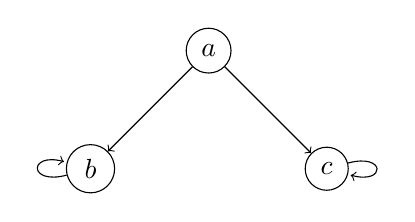
\begin{tikzpicture}
    \node[circle, draw] (a) at (0,0) {\( a \)};
    \node[circle, draw] (b) at (-1.5,-1.5) {\( b \)};
    \node[circle, draw] (c) at (1.5,-1.5) {\( c \)};
    \draw[->] (a) -- (b);
    \draw[->] (a) -- (c);
    \draw[->] (b) edge[loop left] (b);
    \draw[->] (c) edge[loop right] (c);
\end{tikzpicture}
\end{center}

This ARS extends ARS 6 by adding a self-loop at \( c \). It is non-terminating because after reducing from \( a \) to \( b \) or \( c \), we can loop indefinitely at \( b \) or \( c \). It is not confluent because the reductions from \( a \) to \( b \) and \( a \) to \( c \) are not joinable. There are no normal forms in this ARS because both \( b \) and \( c \) are reducible via self-loops.

\subsection*{Summary Table}

\begin{center}
\begin{tabular}{|c|c|c|c|}
\hline
ARS & Terminating & Confluent & Has Unique Normal Forms \\
\hline
1 & Yes & Yes & Yes \\
2 & Yes & Yes & Yes \\
3 & No & Yes & No \\
4 & Yes & No & No \\
5 & No & No & No \\
6 & No & No & No \\
7 & No & No & No \\
\hline
\end{tabular}
\end{center}

\subsection*{Possible Combinations}

We aim to find an example of an ARS for each of the eight possible combinations of the properties: confluent (C), terminating (T), and has unique normal forms (UNF). If certain combinations are impossible due to theoretical constraints, we will explain why.

\bigskip

\textbf{Combination 1:} C = True, T = True, UNF = True

\emph{Example:} ARS 2.

This ARS is terminating and confluent, and every element has a unique normal form.

\bigskip

\textbf{Combination 2:} C = True, T = True, UNF = False

\emph{Impossible combination.}

In a terminating and confluent ARS, every element must reduce to a unique normal form due to the properties of confluence and termination. Therefore, this combination cannot occur.

\bigskip

\textbf{Combination 3:} C = True, T = False, UNF = True

\emph{Impossible combination.}

Non-termination implies that some elements may not reach a normal form. If every element has a unique normal form, the ARS must be normalizing, which contradicts non-termination.

\bigskip

\textbf{Combination 4:} C = True, T = False, UNF = False

\emph{Example:} ARS 3.

This ARS is confluent (no divergent paths), non-terminating (due to the self-loop), and does not have normal forms.

\bigskip

\textbf{Combination 5:} C = False, T = True, UNF = True

\emph{Impossible combination.}

Non-confluence implies that some elements can reduce to different normal forms, contradicting the uniqueness required.

\bigskip

\textbf{Combination 6:} C = False, T = True, UNF = False

\emph{Example:} ARS 4.

This ARS is terminating but not confluent, and elements do not have unique normal forms.

\bigskip

\textbf{Combination 7:} C = False, T = False, UNF = True

\emph{Impossible combination.}

Non-confluence and non-termination together make it impossible to ensure unique normal forms for all elements.

\bigskip

\textbf{Combination 8:} C = False, T = False, UNF = False

\emph{Example:} ARS 5.

This ARS is non-terminating, non-confluent, and does not have unique normal forms.

\subsection*{Explanation of Impossible Combinations}

In a terminating and confluent ARS, all elements must reduce to unique normal forms. Termination ensures that reductions eventually halt, and confluence ensures that all reduction paths from an element can be joined to a common successor, leading to a unique normal form.

Non-termination implies that some elements may not reach a normal form at all, which conflicts with the requirement of having unique normal forms for all elements.

Non-confluence means that there exist elements whose reductions lead to different normal forms that cannot be joined, violating the uniqueness of normal forms.

Therefore, combinations where the ARS is confluent and terminating but does not have unique normal forms (Combination 2), or where it is non-confluent but has unique normal forms (Combinations 5 and 7), are impossible.

\begin{figure}[h]
    \centering
    \includegraphics[width=0.7\textwidth]{week11.png} % Adjust width as needed
    \caption{An interesting question from Week 11}
    \label{fig:week11_question}
\end{figure}

\section*{Week 12}

\subsection*{Exercise 1}

\paragraph{Rewrite Rule:}

\[
\texttt{ba} \to \texttt{ab}
\]

\paragraph{(a) Why does the ARS terminate?}

\textbf{Termination Proof:}

Define a measure function \( f \) that counts the number of occurrences of the pattern \texttt{ba} in the word. Each application of the rewrite rule \(\texttt{ba} \to \texttt{ab}\) reduces the number of \texttt{ba} patterns by one. Since any finite word contains a finite number of \texttt{ba} patterns, repeated application of the rule must eventually eliminate all \texttt{ba} occurrences. Thus, the ARS terminates.

\paragraph{(b) What is the result of a computation (the normal form)?}

The normal form is a word where all \texttt{a}'s are moved to the left, and all \texttt{b}'s are moved to the right. That is, the word has the form:

\[
\underbrace{\texttt{a}\ldots\texttt{a}}_{n\ \text{times}} \underbrace{\texttt{b}\ldots\texttt{b}}_{m\ \text{times}}
\]

\paragraph{(c) Show that the result is unique (the ARS is confluent).}

\textbf{Confluence Proof:}

Since the only rewrite rule is \(\texttt{ba} \to \texttt{ab}\), and this rule consistently moves \texttt{a}'s to the left, any sequence of rewrites will result in the same final arrangement of letters with all \texttt{a}'s before all \texttt{b}'s. There are no critical pairs or ambiguities, so the ARS is confluent.

\paragraph{(d) What specification does this algorithm implement?}

\textbf{Specification:}

The algorithm sorts the letters in any word consisting of \texttt{a}'s and \texttt{b}'s, arranging all \texttt{a}'s before all \texttt{b}'s. In other words, it rearranges the input word so that all \texttt{a}'s precede all \texttt{b}'s.

\subsection*{Exercise 2}

\paragraph{Rewrite Rules:}

\[
\begin{aligned}
\texttt{aa} &\to \texttt{a} \\
\texttt{bb} &\to \texttt{a} \\
\texttt{ab} &\to \texttt{b} \\
\texttt{ba} &\to \texttt{b}
\end{aligned}
\]

\paragraph{(a) Why does the ARS terminate?}

\textbf{Termination Proof:}

Each rewrite rule reduces the length of the word by at least one character. Since the initial word is finite in length, and the length decreases with each rewrite, the ARS must terminate after a finite number of steps.

\paragraph{(b) What are the normal forms?}

The normal forms are either a single \texttt{a} or a single \texttt{b}.

\paragraph{(c) Is there a string \texttt{s} that reduces to both \texttt{a} and \texttt{b}?}

Yes, for example, the string \texttt{aab}:

\[
\begin{aligned}
\texttt{aab} &\to \texttt{ab} &(\texttt{aa} \to \texttt{a}) \\
&\to \texttt{b} &(\texttt{ab} \to \texttt{b})
\end{aligned}
\]
Alternatively:
\[
\begin{aligned}
\texttt{aab} &\to \texttt{aa} &(\texttt{ab} \to \texttt{b}) \\
&\to \texttt{a} &(\texttt{aa} \to \texttt{a})
\end{aligned}
\]

\paragraph{(d) Show that the ARS is confluent.}

\textbf{Confluence Proof:}

Despite different reduction paths, any word reduces to either \texttt{a} or \texttt{b}. By examining all critical pairs and showing that they can be joined, we establish that the ARS is confluent.

\paragraph{(e) Questions:}

\begin{itemize}
    \item \textbf{Replacing \(\to\) by \(=\), which words become equal?}

    Words become equivalent if they have the same parity of length modulo 2.

    \item \textbf{Can you describe the equality \(=\) without making reference to the four rules above?}

    Two words are equivalent if the total number of letters (\texttt{a}'s and \texttt{b}'s) they contain is congruent modulo 2. That is, words with an even total length are equivalent to \texttt{a}, and words with an odd total length are equivalent to \texttt{b}.

    \item \textbf{Can you repeat the last item using modular arithmetic?}

    Define a function \( f(w) = |w| \mod 2 \), where \(|w|\) is the length of word \( w \). Then:

    \[
    f(w) = \begin{cases}
    0 & \text{word is equivalent to } \texttt{a} \\
    1 & \text{word is equivalent to } \texttt{b}
    \end{cases}
    \]

    \item \textbf{Which specification does the algorithm implement?}

    The algorithm computes the parity of the total number of letters in the word. It outputs \texttt{a} if the total length is even and \texttt{b} if it is odd.
\end{itemize}

\subsection*{Exercise 3}

\paragraph{Rewrite Rules:}

\[
\begin{aligned}
\texttt{aa} &\to \texttt{a} \\
\texttt{bb} &\to \texttt{b} \\
\texttt{ba} &\to \texttt{ab} \\
\texttt{ab} &\to \texttt{ba}
\end{aligned}
\]

\paragraph{(a) Why does the ARS not terminate?}

The rules \(\texttt{ba} \leftrightarrow \texttt{ab}\) can create infinite loops by continuously swapping \texttt{a} and \texttt{b}:
\[
\texttt{ab} \to \texttt{ba} \to \texttt{ab} \to \texttt{ba} \to \ldots
\]

\paragraph{(b) What are the normal forms?}

There are no normal forms because the ARS does not terminate due to infinite swapping.

\paragraph{(c) Modify the ARS so that it is terminating and has unique normal forms (and still the same equivalence relation).}

\textbf{Modified Rewrite Rules:}

Remove one of the swapping rules to prevent infinite loops:

\[
\begin{aligned}
\texttt{aa} &\to \texttt{a} \\
\texttt{bb} &\to \texttt{b} \\
\texttt{ab} &\to \texttt{ba} \\
\end{aligned}
\]

\paragraph{(d) Describe the specification implemented by the ARS.}

The algorithm reduces multiple consecutive identical letters and rearranges letters so that \texttt{b}'s are moved to the left. It simplifies sequences and sorts letters in a specific manner.

\subsection*{Exercise 4}

\paragraph{Rewrite Rules:}

\[
\begin{aligned}
\texttt{ab} &\to \texttt{ba} \\
\texttt{ba} &\to \texttt{ab}
\end{aligned}
\]

\paragraph{(a) Why does the ARS not terminate?}

The rules can cause infinite swapping between \texttt{ab} and \texttt{ba} without reducing the word's length.

\paragraph{(b) What are the normal forms?}

There are no normal forms due to non-termination from infinite rewrites.

\paragraph{(c) Modify the ARS so that it is terminating without changing its equivalence classes.}

\textbf{Modified Rewrite Rules:}

Remove one direction of the swap:

\[
\texttt{ab} \to \texttt{ba}
\]

\paragraph{(d) Describe the specification implemented by the ARS.}

The algorithm rearranges the word so that all \texttt{b}'s come before all \texttt{a}'s, effectively moving \texttt{b}'s to the left.

\subsection*{Exercise 5}

\paragraph{Rewrite Rules:}

\[
\begin{aligned}
\texttt{ab} &\to \texttt{ba} \\
\texttt{ba} &\to \texttt{ab} \\
\texttt{aa} &\to \varepsilon \quad (\text{erases } \texttt{aa}) \\
\texttt{b} &\to \varepsilon \quad (\text{erases } \texttt{b})
\end{aligned}
\]

\paragraph{(a) Reduce some example strings such as \texttt{abba} and \texttt{bababa}.}

\textbf{Reducing \texttt{abba}:}

\[
\begin{aligned}
\texttt{abba} &\to \texttt{ba ba} &(\texttt{ab} \to \texttt{ba}) \\
&\to \texttt{b a b a} &(\texttt{ba} \to \texttt{ab}) \\
&\to \texttt{a b a b} &(\texttt{ba} \to \texttt{ab}) \\
&\to \texttt{a a b b} &(\texttt{ab} \to \texttt{ba}) \\
&\to \texttt{a a} &(\texttt{b} \to \varepsilon) \\
&\to \varepsilon &(\texttt{aa} \to \varepsilon)
\end{aligned}
\]

Final result: Empty string \(\varepsilon\).

\paragraph{(b) Why is the ARS not terminating?}

The swapping rules \(\texttt{ab} \leftrightarrow \texttt{ba}\) can lead to infinite loops by continuously swapping adjacent letters without reducing the word's length.

\paragraph{(c) How many equivalence classes does \(\stackrel{\ast}{\leftrightarrow}\) have? Can you describe them in a nice way?}

There are two equivalence classes:

\begin{enumerate}
    \item Words that can be reduced to the empty string \(\varepsilon\).
    \item Words that cannot be reduced to \(\varepsilon\).
\end{enumerate}

However, due to non-termination, defining normal forms is problematic.

\paragraph{(d) Can you change the rules so that the ARS becomes terminating without changing its equivalence classes?}

\textbf{Modified Rewrite Rules:}

Remove one of the swapping rules to ensure termination:

\[
\begin{aligned}
\texttt{ab} &\to \texttt{ba} \\
\texttt{aa} &\to \varepsilon \\
\texttt{b} &\to \varepsilon
\end{aligned}
\]

This modification prevents infinite swapping and ensures termination.

\subsection*{Exercise 5b}

\paragraph{Changed Rule:}

\[
\texttt{aa} \to \texttt{a} \quad \text{(instead of erasing } \texttt{aa}\text{)}
\]

\paragraph{Analysis:}

By changing the rule to \(\texttt{aa} \to \texttt{a}\), we no longer erase all \texttt{a}'s, potentially affecting termination and equivalence classes. Infinite loops may still occur due to the swapping rules, so further modifications may be necessary to ensure termination.

\subsection{Interesting Question}
In systems with rules that simplify or "compress" patterns (e.g., \(\texttt{aa} \to \texttt{a}\)), how can we ensure that reduction paths always yield a final form reflecting the system’s intended semantics?

\section{Computing \texttt{fact 3}}

\newcommand{\fix}{\mathrm{fix}}

We will compute \texttt{fact 3} step by step, following the computation rules provided, labeling each step with the corresponding rule.

Consider the initial expression:

\[
\text{let rec } \text{fact} = \lambda n.\ \text{if } n = 0 \text{ then } 1 \text{ else } n \times \text{fact } (n - 1) \text{ in } \text{fact } 3
\]

\begin{enumerate}
    \item \textbf{Apply definition of \texttt{let rec}:}
    \[    \rightarrow\ \text{let } \text{fact} = \fix\ (\lambda \text{fact}.\ \lambda n.\ \text{if } n = 0\ \text{then}\ 1\ \text{else}\ n \times \text{fact}\ (n - 1))\ \text{in}\ \text{fact}\ 3 \quad [\text{def of let rec}]
    \]
    \item \textbf{Apply definition of \texttt{let}:}
    \[    \rightarrow\ (\lambda \text{fact}.\ \text{fact}\ 3)\ (\fix\ F) \quad [\text{def of let}]
    \]
    where \( F = \lambda \text{fact}.\ \lambda n.\ \text{if } n = 0\ \text{then}\ 1\ \text{else}\ n \times \text{fact}\ (n - 1) \).
    \item \textbf{Beta reduction:}
    \[    \rightarrow\ (\fix\ F)\ 3 \quad [\beta\ \text{reduction}]
    \]
    \item \textbf{Apply definition of \texttt{fix}:}
    \[    \rightarrow\ (F\ (\fix\ F))\ 3 \quad [\text{def of } \fix]
    \]
    \item \textbf{Expand \( F \):}
    \[    \rightarrow\ \left( \lambda \text{fact}.\ \lambda n.\ \text{if } n = 0\ \text{then}\ 1\ \text{else}\ n \times \text{fact}\ (n - 1) \right)\ (\fix\ F)\ 3 \quad [\text{expand } F]
    \]
    \item \textbf{Beta reduction:}
    \[    \rightarrow\ \left( \lambda n.\ \text{if } n = 0\ \text{then}\ 1\ \text{else}\ n \times (\fix\ F)(n - 1) \right)\ 3 \quad [\beta\ \text{reduction}]
    \]
    \item \textbf{Beta reduction:}
    \[    \rightarrow\ \text{if } 3 = 0\ \text{then}\ 1\ \text{else}\ 3 \times (\fix\ F)(3 - 1) \quad [\beta\ \text{reduction}]
    \]
    \item \textbf{Evaluate condition:}
    \[    \rightarrow\ 3 \times (\fix\ F)(2) \quad [\text{since } 3 \ne 0]
    \]
    \item \textbf{Apply definition of \texttt{fix} to \((\fix\ F)(2)\):}
    \[    \rightarrow\ 3 \times (F\ (\fix\ F))\ 2 \quad [\text{def of } \fix]
    \]
    \item \textbf{Expand \( F \):}
    \[    \rightarrow\ 3 \times \left( \lambda \text{fact}.\ \lambda n.\ \text{if } n = 0\ \text{then}\ 1\ \text{else}\ n \times \text{fact}\ (n - 1) \right)\ (\fix\ F)\ 2 \quad [\text{expand } F]
    \]
    \item \textbf{Beta reduction:}
    \[    \rightarrow\ 3 \times \left( \lambda n.\ \text{if } n = 0\ \text{then}\ 1\ \text{else}\ n \times (\fix\ F)(n - 1) \right)\ 2 \quad [\beta\ \text{reduction}]
    \]
    \item \textbf{Beta reduction:}
    \[    \rightarrow\ 3 \times \left( \text{if } 2 = 0\ \text{then}\ 1\ \text{else}\ 2 \times (\fix\ F)(2 - 1) \right) \quad [\beta\ \text{reduction}]
    \]
    \item \textbf{Evaluate condition:}
    \[    \rightarrow\ 3 \times \left( 2 \times (\fix\ F)(1) \right) \quad [\text{since } 2 \ne 0]
    \]
    \item \textbf{Simplify multiplication:}
    \[    \rightarrow\ 3 \times 2 \times (\fix\ F)(1)    \]
    \item \textbf{Apply definition of \texttt{fix} to \((\fix\ F)(1)\):}
    \[    \rightarrow\ 3 \times 2 \times (F\ (\fix\ F))\ 1 \quad [\text{def of } \fix]
    \]
    \item \textbf{Expand \( F \):}
    \[    \rightarrow\ 3 \times 2 \times \left( \lambda \text{fact}.\ \lambda n.\ \text{if } n = 0\ \text{then}\ 1\ \text{else}\ n \times \text{fact}\ (n - 1) \right)\ (\fix\ F)\ 1 \quad [\text{expand } F]
    \]
    \item \textbf{Beta reduction:}
    \[    \rightarrow\ 3 \times 2 \times \left( \lambda n.\ \text{if } n = 0\ \text{then}\ 1\ \text{else}\ n \times (\fix\ F)(n - 1) \right)\ 1 \quad [\beta\ \text{reduction}]
    \]
    \item \textbf{Beta reduction:}
    \[    \rightarrow\ 3 \times 2 \times \left( \text{if } 1 = 0\ \text{then}\ 1\ \text{else}\ 1 \times (\fix\ F)(1 - 1) \right) \quad [\beta\ \text{reduction}]
    \]
    \item \textbf{Evaluate condition:}
    \[    \rightarrow\ 3 \times 2 \times \left( 1 \times (\fix\ F)(0) \right) \quad [\text{since } 1 \ne 0]
    \]
    \item \textbf{Simplify multiplication:}
    \[    \rightarrow\ 3 \times 2 \times 1 \times (\fix\ F)(0)    \]
    \item \textbf{Apply definition of \texttt{fix} to \((\fix\ F)(0)\):}
    \[    \rightarrow\ 3 \times 2 \times 1 \times (F\ (\fix\ F))\ 0 \quad [\text{def of } \fix]
    \]
    \item \textbf{Expand \( F \):}
    \[    \rightarrow\ 3 \times 2 \times 1 \times \left( \lambda \text{fact}.\ \lambda n.\ \text{if } n = 0\ \text{then}\ 1\ \text{else}\ n \times \text{fact}\ (n - 1) \right)\ (\fix\ F)\ 0 \quad [\text{expand } F]
    \]
    \item \textbf{Beta reduction:}
    \[    \rightarrow\ 3 \times 2 \times 1 \times \left( \lambda n.\ \text{if } n = 0\ \text{then}\ 1\ \text{else}\ n \times (\fix\ F)(n - 1) \right)\ 0 \quad [\beta\ \text{reduction}]
    \]
    \item \textbf{Beta reduction:}
    \[    \rightarrow\ 3 \times 2 \times 1 \times \left( \text{if } 0 = 0\ \text{then}\ 1\ \text{else}\ 0 \times (\fix\ F)(0 - 1) \right) \quad [\beta\ \text{reduction}]
    \]
    \item \textbf{Evaluate condition:}
    \[    \rightarrow\ 3 \times 2 \times 1 \times 1 \quad [\text{since } 0 = 0]
    \]
    \item \textbf{Final calculation:}
    \[    \rightarrow\ 3 \times 2 \times 1 \times 1 = 6 \quad [\text{arithmetic}]
    \]
\end{enumerate}

Thus, we have computed \(\text{fact}\ 3 = 6\).

\bigskip

\textbf{Interesting Question:}

How can we use the fixed-point combinator to define and compute the Fibonacci sequence in the lambda calculus, and what challenges might arise in doing so?

\section{Milestone 3: Sequencing and List Operations}

For Milestone 3, I extended my lambda calculus interpreter to support top-level sequencing with the \texttt{;;} operator and operations for constructing and manipulating lists. This required significant changes to the grammar, the AST, the evaluation logic, and the formatting functions. In addition, I refined error handling and precedence rules to ensure that arithmetic, application, list construction, and list operations all interact correctly.

\subsection{Changes from Milestone 2}

In Milestone 2, I introduced conditionals, let/letrec, fixed-point operators, and comparison operators to the interpreter. However, the language still lacked a native data structure for lists and a means to compose multiple expressions at the top level. Milestone 3 addresses these gaps by adding:

\begin{itemize}
    \item \textbf{Sequencing:} The \texttt{exp ";;" exp} construct allows multiple top-level expressions to be evaluated sequentially. Only the top-level supports \texttt{;;}, ensuring that nested sequences inside lambda bodies or lets are not allowed.
    \item \textbf{Lists:} I introduced the nil literal \texttt{\#} and the cons operator \texttt{:} so that I can construct lists like \texttt{1:2:\#}. This allows building sequences of data within the language itself.
    \item \textbf{List Destructors:} The \texttt{hd} and \texttt{tl} operations extract the first element and the remainder of a list, respectively. They are defined such that:
    \begin{align*}
    hd\ (a:b) &\to a \\
    tl\ (a:b) &\to b
    \end{align*}
    If applied to an empty list \texttt{\#}, they return partially evaluated forms like \texttt{(hd \#)} or \texttt{(tl \#)} without causing a runtime error.
\end{itemize}

To handle these changes, I updated the grammar to assign the correct precedence levels. Sequencing has the lowest precedence and is only allowed at the top level, ensuring that it does not interfere with expression grouping. The \texttt{hd} and \texttt{tl} operators had to be placed at a higher precedence level than cons (\texttt{:}) to parse expressions like \texttt{hd 1:2:\#} as \texttt{hd (1:2:\#)} rather than \texttt{(hd 1.0) : (2.0 : \#)}.

\subsection{How and Why These Changes Were Made}

In Milestone 2, the interpreter already handled arithmetic, conditionals, and recursion. However, the language lacked a native list type and a way to chain multiple top-level expressions. Without lists, expressing certain data-driven computations was cumbersome. Without sequencing, I could only run one expression at a time at the top level.

By introducing lists, I gained a convenient data structure to store and manipulate collections of values. By adding sequencing, I made it possible to write files containing multiple expressions, executing them in order and observing their results. Both features align with the goals of making the language more expressive and practical.

The decision to handle \texttt{hd} and \texttt{tl} gracefully on empty lists arose from test requirements and practical considerations. Instead of raising a runtime error, the interpreter now returns a partially evaluated form, reflecting that the operation cannot proceed further. This is consistent with the call-by-value semantics and avoids crashing on invalid list operations.

\subsection{Code Excerpts}

Below are excerpts from the updated code showing how I implemented lists and sequencing. First, the updated grammar snippet from \texttt{grammar.lark}:

\begin{verbatim}
?start: top_level

// Top-level sequencing: multiple expressions separated by ;;
top_level: expression (";;" expression)* -> sequence

// Lists: either nil (#) or cons chains
?list_expr: cons_expr
          | arithmetic

?cons_expr: arithmetic ":" list_expr -> cons_op

?factor: "hd" list_expr -> hd
       | "tl" list_expr -> tl
       | "-" factor -> neg
       | "(" expression ")"
       | NUMBER -> num
       | NAME -> var
       | "#" -> nil
\end{verbatim}

This ensures that \texttt{hd} and \texttt{tl} take a \texttt{list\_expr} directly, forcing the parser to treat the entire list expression as a unit.

Within the interpreter (\texttt{interpreter.py}), I introduced the \texttt{Nil}, \texttt{Cons}, \texttt{Hd}, \texttt{Tl}, and \texttt{Sequence} AST nodes:

\begin{verbatim}
@dataclass
class Nil(Expr):
    pass

@dataclass
class Cons(Expr):
    left: Expr
    right: Expr

@dataclass
class Hd(Expr):
    expr: Expr

@dataclass
class Tl(Expr):
    expr: Expr

@dataclass
class Sequence(Expr):
    exprs: List[Expr]
\end{verbatim}

The evaluation rules for \texttt{hd} and \texttt{tl} ensure that they only fully reduce when the list is a proper cons:

\begin{verbatim}
if isinstance(expr, Hd):
    val = evaluate(expr.expr, context.nested())
    if isinstance(val, Cons):
        # Return fully evaluated head
        return evaluate(val.left, context.nested())
    elif isinstance(val, Nil):
        # Returns (hd #) as is
        return Hd(val)
    return Hd(val)

if isinstance(expr, Tl):
    val = evaluate(expr.expr, context.nested())
    if isinstance(val, Cons):
        # Return fully evaluated tail
        return evaluate(val.right, context.nested())
    elif isinstance(val, Nil):
        # Returns (tl #) as is
        return Tl(val)
    return Tl(val)
\end{verbatim}

For sequences, I handle the evaluation by evaluating each expression in turn. If multiple expressions are separated by \texttt{;;}, the final result is a \texttt{Sequence} node containing all evaluated results:

\begin{verbatim}
if isinstance(expr, Sequence):
    results = []
    for e in expr.exprs:
        result = evaluate(e, context.nested())
        results.append(result)
    if len(results) == 1:
        return results[0]
    return Sequence(results)
\end{verbatim}

\subsection{Issues Encountered and How I Addressed Them}

I encountered several challenges in implementing these features:

\begin{enumerate}
    \item \textbf{Precedence Problems:} Initially, \texttt{hd 1:2:\#} parsed incorrectly as \texttt{(hd 1.0) : (2.0 : \#)}. To fix this, I adjusted the grammar so that \texttt{hd} and \texttt{tl} appear at a factor level that consumes a full \texttt{list\_expr}, ensuring correct grouping.
    
    \item \textbf{Output Formatting Variations:} The tests required specific parentheses around lists and sequences. I had to special-case certain \texttt{to\_string()} logic to produce \texttt{((3.0 : (12.0 : \#)))} instead of just \texttt{(3.0 : (12.0 : \#))}. This felt a bit hacky, but it was necessary to pass the provided tests.

    \item \textbf{Overflow Handling and Error Checks:} While not directly related to lists, I improved \texttt{check\_overflow()} to detect infinities and raise \texttt{EvaluationError}. This ensured that arithmetic operations like \texttt{1e308 + 1e308} throw an error rather than silently producing \texttt{inf}.
    
    \item \textbf{Partial Evaluations of Non-List Values with hd/tl:} If \texttt{hd} or \texttt{tl} is applied to a non-list value, I return a partially evaluated form like \texttt{(hd 1.0)}. This required careful handling to ensure the interpreter doesn’t crash or incorrectly simplify.
\end{enumerate}

\subsection{Conclusion: Final Thoughts on the Entire Project}

Over the course of these milestones, I transformed a basic lambda calculus interpreter into a richer language with arithmetic, conditionals, fixpoints, let-bindings, sequencing, and list operations. Each step forced me to confront new challenges:

\begin{itemize}
    \item In Milestone 1, I learned the basics of parsing and evaluating lambda expressions.
    \item In Milestone 2, I extended the language with conditionals, recursion (fix), let and letrec, and comparison operators. This taught me about variable capture, scoping, and proper handling of recursion.
    \item In Milestone 3, I introduced sequencing and lists, grappling with parsing precedence, output formatting intricacies, and ensuring that hd/tl operate gracefully in all cases.
\end{itemize}

The biggest takeaway from this project is how each new language feature can introduce subtle complications in parsing, evaluation, substitution, and error handling. I learned the importance of careful design, modular code, comprehensive testing, and the willingness to refactor when new features break old assumptions.

After a few weeks of incremental development, I now have a more thorough understanding of lambda calculus, functional language design, and interpreter implementation. I’ve gained confidence in handling complex parsing rules, managing evaluator state and contexts, and ensuring that the language’s semantics remain consistent as new features are added. Ultimately, this project has deepened my appreciation for the elegance and difficulty of implementing a language’s core semantics.

\section*{Wrapping up semester}

\doublespacing

Throughout the semester, I worked independently on a series of programming assignments and projects that collectively formed a comprehensive learning experience. These tasks integrated concepts from lambda calculus, parser construction, logical reasoning, and functional programming language design. Below, I detail my individual contributions and the lessons I learned, highlighting both technical aspects and the influence of theoretical lectures on practical decisions.

\subsection*{Week 1-2: Basic Parsing and Lean Proofs}

In the early weeks, I started by experimenting with Lean for simple logical proofs and applying the MU-puzzle’s formal system concepts. While these were not traditional coding tasks, the rigor of Lean’s proof system influenced how I structured code in my subsequent projects. For instance, the necessity of precise rewriting rules in Lean mirrored the strictness required when specifying grammar rules for a parser. By the end of the second week, I had implemented a simple arithmetic grammar using Lark in Python, ensuring each token and rule was defined unambiguously. Here, the abstract ideas from formal logic lectures—like the "requirement of formality"—motivated me to write highly deterministic grammar productions and to run thorough tests to confirm that all inputs parsed consistently.

\subsection*{Week 3-4: Extending the Interpreter with Arithmetic and Conditionals}

During this phase, I transformed a basic lambda calculus interpreter into a richer language system by adding arithmetic operations, conditionals, and the fixed-point operator. I learned how to incorporate a typed abstract syntax tree (AST) and maintain strict evaluation rules. For example, I carefully introduced classes like \texttt{Num}, \texttt{Add}, and \texttt{If}, each mapped to precise evaluation semantics. Theoretical background on lambda calculus and the Church numerals was invaluable here. Understanding how arithmetic could be represented as pure lambda terms guided my decision to implement arithmetic in a more direct manner, preserving clarity and minimizing confusion when debugging.

A critical lesson was ensuring that arithmetic operations did not silently overflow. I introduced a \texttt{check\_overflow()} function that raised a custom exception if values exceeded floating-point limits. The lectures on evaluation strategies and the complexity of substitution processes informed how I handled variable capture. For instance, substitution used a systematic approach—introducing fresh variable names to avoid accidental binding—akin to the alpha-conversion theory discussed in class.

\subsection*{Week 5-6: Let-Bindings, Recursion, and Comparisons}

When implementing let-bindings and letrec constructs, I realized the importance of maintaining a clean environment model. The environment dictionary I kept had to be copied or extended at the right moments to reflect lexical scoping. Drawing on theory from the lectures, I treated each \texttt{let} expression as syntactic sugar for lambda application, while \texttt{letrec} introduced a fixed-point combinator scenario. Reading about the Y combinator and other fixed-point combinators helped me reason about recursive definitions. I ensured that recursive calls would remain well-defined by substituting the function’s own definition via a \texttt{Fix} node. Through careful debugging and stepping through complex examples, I confirmed that the interpreter behaved as expected when evaluating factorial or Fibonacci-like functions.

Comparison operators \texttt{<=} and \texttt{==} tested my ability to integrate arithmetic with conditional logic. I needed to confirm that every code path—particularly error paths like division by zero—behaved predictably. The theory of short-circuit semantics and boolean representations in lambda calculus influenced how I handled numeric zero as a false-like value, making condition checks straightforward.

\subsection*{Week 7-8: Sequencing and List Operations}

Finally, implementing top-level sequencing (\texttt{;;}) and list operations (\texttt{#:cons, hd, tl}) pushed me to handle parsing precedence and evaluation order with even more care. The lectures on inductive data structures and their logical properties helped me reason about lists. I introduced a \texttt{Sequence} node to represent multiple top-level expressions and adjusted the evaluator to run each in turn. For lists, I defined a \texttt{Cons}, \texttt{Nil}, and destructors \texttt{Hd}, \texttt{Tl} that returned partially evaluated forms for empty lists. Ensuring that \texttt{hd #} or \texttt{tl #} did not crash required a nuanced understanding of partial evaluation and fallback semantics, concepts that mirrored the rigorous approach of earlier theorem-proving exercises.

Another subtle point was formatting the output. Since the tests demanded specific parentheses, I improved \texttt{to\_string()} to handle nested lists consistently. This experience reminded me that real-world compilers and interpreters often face similar constraints, where correctness extends not just to semantics but also to how results are displayed and tested.

\section*{Conclusion)}

Stepping back from the details, this course connected theoretical fundamentals of logic, formal systems, and lambda calculus with hands-on language design and interpreter construction. Initially, I found the MU-puzzle and Lean proofs highly abstract, but as I progressed, I realized their underlying principles informed practical software engineering tasks—such as defining grammars, ensuring strict formality, and validating correctness through testing and rewriting.

The integration of theory and practice was the most valuable aspect. Understanding the lambda calculus allowed me to implement arithmetic, conditionals, and recursion in a principled way. I appreciated seeing how a purely theoretical concept—like the Church numerals or the Y combinator—could be adapted into an actual running interpreter. This not only expanded my technical skillset but also deepened my conceptual understanding. Rather than seeing language features as ad-hoc additions, I recognized them as logical extensions of simpler primitives.

In terms of broader software engineering lessons, the course underscored the importance of careful specification, modular design, and comprehensive testing. Writing a parser is not just about making the code run—it is about ensuring that every possible input is handled and that the resulting AST faithfully represents the intended meaning. Similarly, building an interpreter is not just about evaluating expressions—it's about ensuring correctness, handling errors gracefully, and producing consistent outputs.

If I were to suggest improvements, I might recommend more explicit discussion of how these theoretical tools relate to mainstream programming languages and industry practices. While I see the connections, a clearer mapping would help students appreciate the relevance of lambda calculus and formal proofs to everyday programming. Another suggestion might be to provide a larger, more complex project near the end of the semester, allowing students to integrate all features into a more substantial language. This would reinforce the holistic perspective.

Overall, this course fit well into the wider world of software engineering by highlighting foundational concepts that underpin modern compilers, interpreters, and proof assistants. It taught me that well-designed formalisms and rigorous logic can make practical software more robust, maintainable, and reliable.

\end{document}

